%   MSc Business Analytics Dissertation
%   Format based on skeleton template provided as part of module MIS40750
%
%   Title:     Optimising the design of buffer preparation in bioprocessing
%              facilities
%   Author:    Sean Tully
%
%   Chapter 6: Discussion
%
%   Change Control:
%   When     Who   Ver  What
%   -------  ----  ---  --------------------------------------------------------
%   06Jun16  ST    0.1  Begun 
%

\chapter{Discussion}\label{C.discussion}

\begin{quote}
Nothing in life is as important as you think it is when you are thinking about
it.

\hspace{2cm}--- Daniel Kahneman,
\emph{Thinking, Fast and Slow}
\end{quote}

\section{Comment on Results}\label{S.rescomment}
The results obtained show that the model is suitable for generating optimal
buffer preparation designs.
For problem sizes in the expected range of 10--20 buffers, it is important to
note that an exact solution can be obtained in a reasonable amount of time.
This is an important result; prior to carrying out this exercise, it was not
known if an optimum solution could feasibly be obtained.

The use of the proprietary CPLEX solver produced the fastest solutions and
produced a feasible solution for all problems examined.
The Cbc solver was less robust; on several occasions it crashed while running.
The worst performance was obtained from the GLPK solver, which appears incapable
of arriving at an optimum solution in under an hour for a medium sized problem.

\section{Challenges}\label{S.challenges}
The most challenging part of this study was the development of the constraint
equations required for the complete model, particularly in the area of cyclic
task scheduling.  The PuLP API is easy to use and well documented, so building
the model in python was a more straightforward task.

\section{Complexity}\label{S.complexity}
The notation for complexity in this section is according to \citet{Knuth:1976}.

The problem complexity depends on both the number of buffers, $N$,
and the number of vessels, $M$.
The complexity may be evaluated in terms of both the number of variables and
the number of equations in the problem.
The complexities of the basic and complete problems are summarised in
\hyperref[tbl.complexity]{Table \ref*{tbl.complexity}}.
For example, a complete problem with twelve buffers and twelve vessels has
\num{2281} equations in \num{1206} variables.
\begin{table}[t]
    \centering
    \caption{Model complexity}
    \label{tbl.complexity}
    \small
    \begin{tabular}{l | c | c}
        model & no. of variables & no. of equations \\ \hline
        basic & $N^2 + NM$ & $2N^2 + 3N + 1$\\
        complete & $N {{N}\choose{2}} + N^2 + {{N}\choose{2}} + NM + 5N$
        & $2N{{N}\choose{2}} + 4{{N}\choose{2}} + 2N^2 + 12N + 1$\\
    \end{tabular}
\end{table}
\begin{table}[t]
    \centering
    \caption{Simplified model complexity}
    \label{tbl.complexity2}
    \begin{tabular}{l | c | c}
        model & no. of variables & no. of equations\\ \hline
        basic & $2N^2$ & $2N^2 + 3N + 1$\\
        complete & $\tfrac{1}{2} N^{3} + \tfrac{5}{2} N^{2} + 5 N$
            & $N^{3} + 4 N^{2} + 12 N + 1$\\
    \end{tabular}
\end{table}

Noting that there is a weak dependence on $M$ and that, as the problem
grows larger in terms of $N$, it is likely that $M$ will
reach a maximum value, the approximation $M \approx N$ may
be used as a conservative simplification when considering complexity.
This simplification has been used to generate the plots in 
Figures \ref{fig.dims} and \ref{fig.eqns}.
The complexity can be further simplified by noting that for the binomial
coefficient term, 
\begin{equation}
    \lim_{N\to\infty}{{N}\choose{2}} = \tfrac{1}{2} N^{2}
\end{equation}
Applying both approximations gives the simplified complexities tabulated in
\hyperref[tbl.complexity2]{Table \ref*{tbl.complexity2}}.

For the basic model, we can see that both the number of variables and the
number of equations is $O \left( N^2 \right)$.

For the complete model, the number of variables and the number of equations
are both $O \left( N^3 \right)$.

The addition of the scheduling constraints in the complete model requires the
comparison of pairs of buffers, which is $O \left( N^2 \right)$. 
These comparisons occur for each slot, giving a multiplicative factor of 
$O \left( N \right)$, leading to an overall complexity of
$O \left( N^3 \right)$.

As was mentioned in \hyperref[SS.solvers]{Section \ref*{SS.solvers}}, the time
complexity of the complete problem is exponential in $N$, which indicated the
complete model is \textbf(NP)-hard.
It was noted in \hyperref[S.intro4]{Section \ref*{S.intro4}}
that the problem appeared to bear similarities to the
bin-packing problem, which is also known to be \textbf{NP}-hard
\citep{Korte:2012}, so this result was as expected.


\begin{figure}
    \centering
    \includegraphics[width=\linewidth]{./figures/variables.pdf}
    \caption{Model complexity -- variables}
    \label{fig.dims}
\end{figure}
\begin{figure}
    \centering
    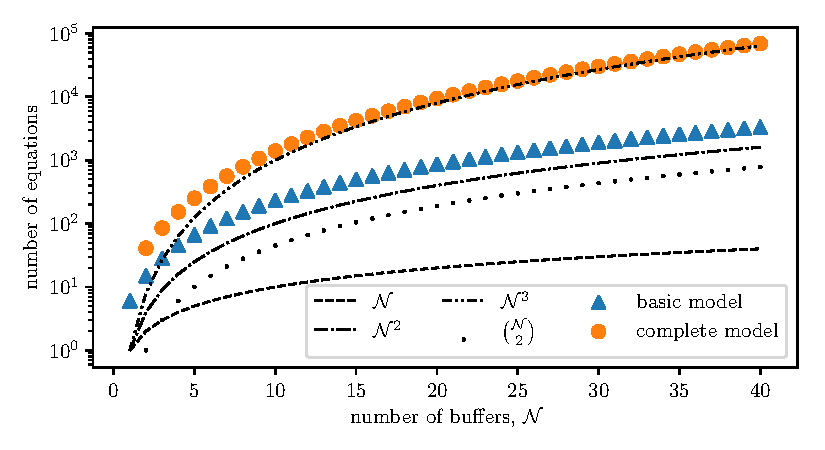
\includegraphics[width=\linewidth]{./figures/equations.pdf}
    \caption{Model complexity -- equations}
    \label{fig.eqns}
\end{figure}
